\phantomsection\numberedsection{RF1.9 Crear informe de cuenta}

\subsection*{Descripción}
El sistema muestra un informe detallado con la información de la cuenta, incluyendo el
nombre de la cuenta, fecha y hora de creación, número de productos, categorías 
de producto, atributos de usuario y relaciones creadas.

\vspace{0.15cm}

\textbf{Pre-condición}\par
El usuario ha iniciado sesión en Mini PIM y es la cuenta Owner.\par
\vspace{0.15cm}

\textbf{Post-condición}
\begin{itemize}
    \item Caso de éxito: El sistema muestra el informe detallado de la cuenta.
    \item Caso mínimo: El sistema notifica al usuario el resultado al crear el informe: exitosa o fallida.
\end{itemize}

\textbf{Prioridad:}
Baja
\vspace{0.15cm}

\textbf{Autores: }
Francisco Javier Jordá Garay y Janine Olegario.\par
\vspace{0.15cm}

\textbf{Control de cambios: } Versión 1: Definición del caso de uso

\numberedsubsection{Escenario principal}
\begin{enumerate}
    \item El usuario\footnote{El usuario en este caso de uso es un Owner. Se detalló en el DGR que el Owner tiene la cuenta principal de la empresa, y el informe de cuenta es único por cuenta} ha iniciado sesión con su cuenta Owner.
    \item El usuario accede a la sección \enquote{Cuenta}\footnote{Esta sección no es un apartado en el Dashboard, sino un botón circular con icono de usuario en la esquina superior derecha.}.
    \item El sistema genera automáticamente el informe con los datos de la cuenta del usuario.
    \item El sistema muestra al usuario el informe completo con los siguientes datos:
        \begin{itemize}
            \item Nombre de la cuenta.
            \item Fecha y hora de creación de la cuenta.
            \item Número de productos de la cuenta.
            \item Número de categorías de productos creadas (máximo 3).
            \item Número de atributos de usuario creados (máximo 5).
            \item Número de relaciones creadas (máximo 3).
        \end{itemize}
\end{enumerate}

\newpage % para que se pueda leer bien la footnote

\numberedsubsection{Escenarios alternativos}
\begin{description}        
    \item[4.a] El sistema intenta generar el informe, pero se produce un error interno.
    \begin{enumerate}
        \item[4.a.1] El sistema muestra un mensaje de error indicando que no se pudo generar el informe y regresa al usuario a la sección donde estaba anteriormente.\footnote{El usuario puede acceder al informe de su cuenta desde cualquier apartado del sistema, entonces si no puede acceder a su informe de cuenta es regresado a donde estaba trabajando previamente.}
    \end{enumerate}
\end{description}

\numberedsubsection{Casos de Prueba}
\underline{Escenario: Principal}\par
\vspace{0.15cm}
\textbf{Dado} que el usuario ha iniciado sesión con su cuenta Owner,\par
\textbf{Y} se encuentra en la sección \enquote{Cuenta},\par
\textbf{Cuando} el usuario accede al apartado de informe de cuentas,\par
\textbf{Entonces} genera automáticamente el informe automáticamente el informe de cuenta,\par 
\textbf{Y} el sistema muestra el informe completo con los siguientes datos:\par
\begin{itemize}
    \item Nombre de la cuenta.
    \item Fecha y hora de creación de la cuenta.
    \item Número de productos de la cuenta.
    \item Número de categorías de productos creadas (máximo 3).
    \item Número de atributos de usuario creados (máximo 5).
    \item Número de relaciones creadas (máximo 3).
\end{itemize}
\vspace{0.20cm}


\underline{Escenario: Alternativo 4.a}\par
\vspace{0.15cm}
\textbf{Dado} que el usuario ha iniciado sesión con su cuenta Owner,\par
\textbf{Y} se encuentra en la sección \enquote{Cuenta},\par
\textbf{Cuando} el usuario accede al apartado de informe de cuentas,\par 
\textbf{Y} ocurre un error interno del sistema mientras se genera el informe,\par
\textbf{Entonces} el sistema muestra un mensaje de error indicando que no se pudo generar el informe,\par
\textbf{Y} redirige al usuario a la sección donde estaba anteriormente.\par
\vspace{0.20cm}

\newpage % Muestra los bocetos en una nueva página

\numberedsubsection{Bocetos}
\begin{figure}[H]
    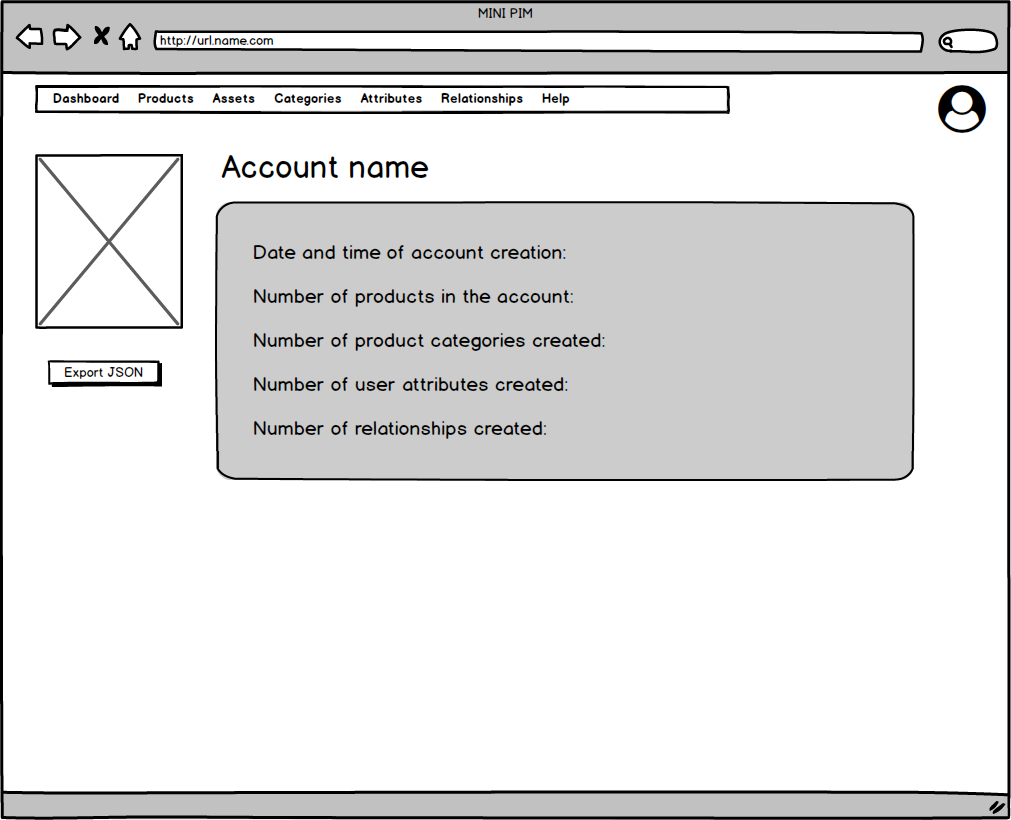
\includegraphics[width=1\linewidth]{assets/mockups/RF1.9CrearInformeCuenta.png}
    \caption{Informe de Cuentas generado en sección \enquote{Cuenta}}
   \end{figure}
\vspace{1.0cm}

\newpage % Muestra el diagrama de secuencias en una nueva página

\numberedsubsection{Diagrama de Secuencia}
\begin{figure}[H]
    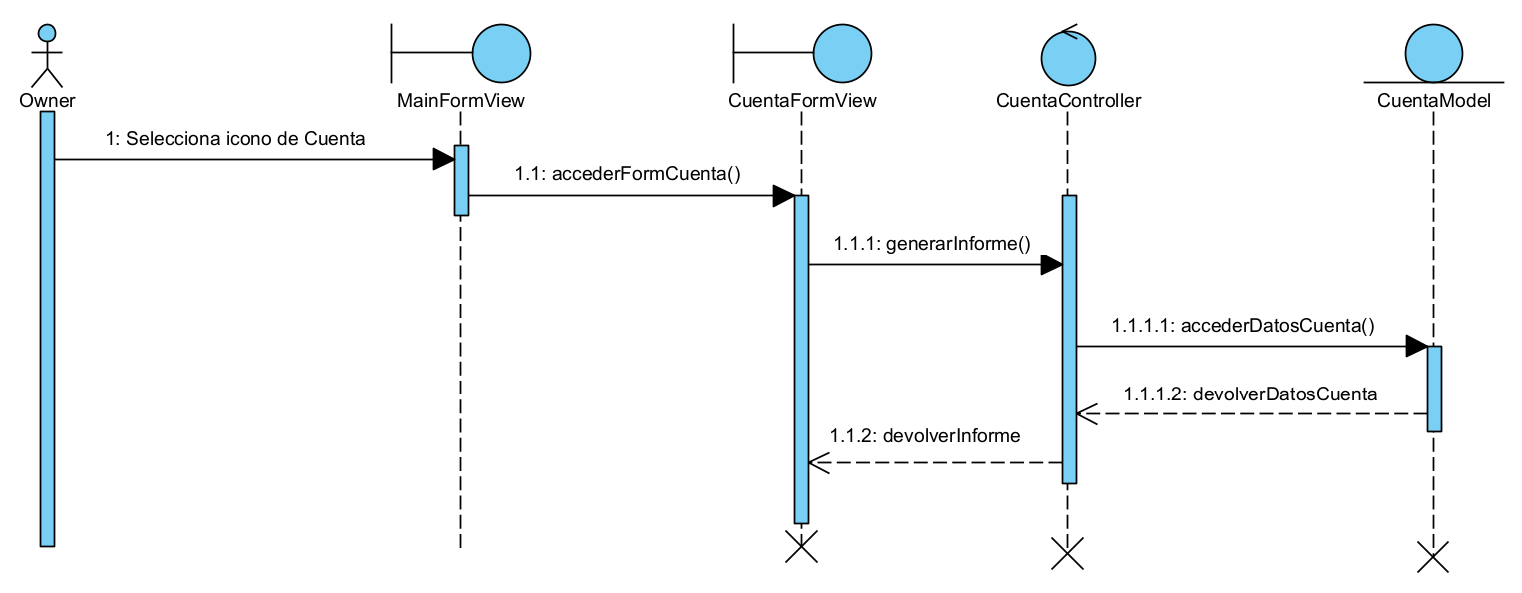
\includegraphics[width=1\linewidth]{assets/sequence/RF1.9_CrearInformeCuenta_v5.png}
    \caption{Escenario principal para crear el Informe de Cuenta}
   \end{figure}
\vspace{1.0cm}

\newpage % Inicia en una nueva página otro caso de uso